\subsection{Exercises}

%%%%%%%%%%%%%%%%%%%%%%%%%%%%%%
\Large{Problem 4.1}
\begin{figure}[H]
    \centering
    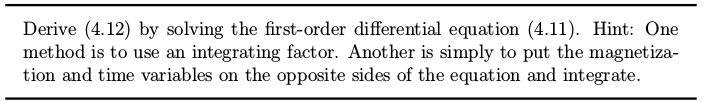
\includegraphics[width=0.8\textwidth,keepaspectratio]{prbl41}
    \label{fig:prbl41}
\end{figure}

\begin{figure}[H]
    \centering
    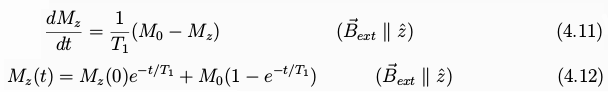
\includegraphics[width=0.8\textwidth,keepaspectratio]{form411412}
    \label{fig:form411412}
\end{figure}

\textit{Remember:}
\begin{itemize}
	\item After applying an RF pulse, the longitudinal magnetization 
	relaxes back to its equilibrium value ($M_0$), following an 
	exponential evolution from the initial value ($M_z(0)$).
\end{itemize}

\textit{Proof.}

\begin{flalign*}
    \frac{d M_z}{dt} &= \frac{1}{T_1} (M_0 - M_z) \\ 
    \frac{1}{M_0 - M_z} d M_z &= \frac{1}{T_1} dt \\
    \int_{M_z(0)}^{M_z(t)} \frac{1}{M_0 - M_z}d M_z &= \int_{t}^{0} \frac{1}{T_1} dt \\
    [ln(M_0 - M_z)]_{M_z(0)}^{M_z(t)} &= [\frac{t}{T_1}]_{t}^{0} \\
    ln \frac{M_0 - M_z(t)}{M_0 - M_z(0)} &= - \frac{t}{T_1} \\
    exp(ln \frac{M_0 - M_z(t)}{M_0 - M_z(0)}) &= exp (- \frac{t}{T_1}) \\
    \frac{M_0 - M_z(t)}{M_0 - M_z(0)} &= exp (- \frac{t}{T_1}) \\
    M_0 - M_z(t) &= M_0 \, e^{-t/T_1} - M_z(0) \, e^{-t/T_1} \\
    M_z(t) &= M_0 (1 - e^{-t/T_1}) + M_z(0) e^{-t/T_1}
\end{flalign*}

\clearpage
%%%%%%%%%%%%%%%%%%%%%%%%%%%%%%
\Large{Problem 4.2}
\begin{figure}[H]
    \centering
    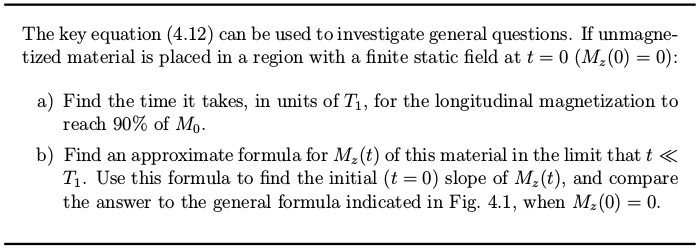
\includegraphics[width=0.8\textwidth,keepaspectratio]{prbl42}
    \label{fig:prbl42}
\end{figure}

\textit{Remember:}
\begin{itemize}
	\item Investigating general questions using $M_z(t) = M_z(0) e^{-t/T_1} + M_0 (1 - e^{-t/T_1})$
    \item \textit{Taylor Series}: \\
    $f(x) = f(a) + \frac{f'(a)}{1!} (x-a) + \frac{f''(a)}{2!} (x-a)^2 + \frac{f'''(a)}{3!} (x-a)^3 + ...$ \\
    \item \textit{Maclaurin Series} (is Taylor series for $a=0$): \\
    $f(x) = f(0) + \frac{f'(0)}{1!} x + \frac{f''(0)}{2!} x^2 + \frac{f'''(0)}{3!} x^3 + ...$ \\
    \item If $f(x) = e^{-t/T_1}$, then: $e^{-t/T_1} \approx 1 - \frac{t}{T_1} $ 
\end{itemize}

\textit{a) Proof.}\\
\textit{We know that:}\\
\begin{flalign*}
    M_z(t) &= 0.9 M_0 \\
    M_z(0) &= 0
\end{flalign*}

\textit{Therefore:}
\begin{flalign*}
    M_z(t) &= M_z(0) e^{-t/T_1} + M_0 (1 - e^{-t/T_1}) \\
    0.9 M_0 &= M_0 (1 - e^{-t/T_1}) \\
    e^{-t/T_1} &= 0.1 \\
    -t/T_1 &= ln(0.1) \\
    t &= 2.3 \, T_1
\end{flalign*}

\textit{b) Proof.}\\
\textit{We know that:}\\
\begin{flalign*}
    t \, << \, T_1
\end{flalign*}

\textit{Therefore:}
\begin{flalign*}
    M_z(t) &= M_z(0) e^{-t/T_1} + M_0 (1 - e^{-t/T_1}) \\
    [\frac{dM_z(t)}{dt}]_{t<<T_1} &= - [\frac{1}{T_1} M_z(0) e^{-t/T_1}]_{t<<T_1} + [\frac{1}{T_1} M_0 e^{-t/T_1}]_{t<<T_1} \\
    [\frac{dM_z(t)}{dt}]_{t<<T_1} &= - \frac{1}{T_1} M_z(0) + \frac{1}{T_1} M_0 \\
    [\frac{dM_z(t)}{dt}]_{t<<T_1} &= \frac{1}{T_1} ( M_0 - M_z(0) ) 
\end{flalign*}

\clearpage
%%%%%%%%%%%%%%%%%%%%%%%%%%%%%%
\Large{Problem 4.3}
\begin{figure}[H]
    \centering
    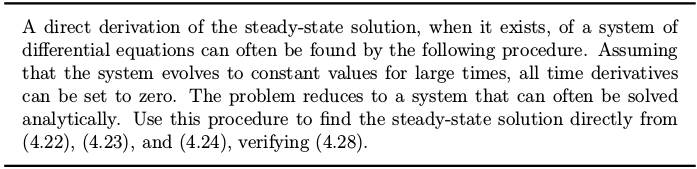
\includegraphics[width=0.8\textwidth,keepaspectratio]{prbl43}
    \label{fig:prbl43}
\end{figure}

\textit{Remember:}
\begin{itemize}
	\item Finding the steady-state solution.
\end{itemize}

\begin{figure}[H]
    \centering
    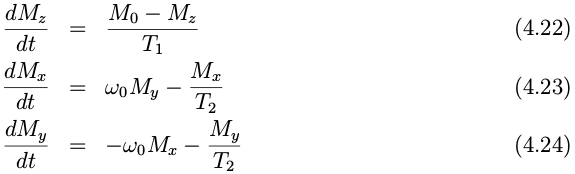
\includegraphics[width=0.8\textwidth,keepaspectratio]{form422423424}
    \label{fig:form422423424}
\end{figure}
\begin{figure}[H]
    \centering
    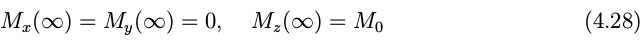
\includegraphics[width=0.8\textwidth,keepaspectratio]{form428}
    \label{fig:form428}
\end{figure}

\textit{Proof.}
\begin{flalign*}
    \frac{M_0 - M_z}{T_1} &= 0 \\
    \omega_0 M_y - \frac{M_x}{T_2} &= 0 \\
    - \omega_0 M_x - \frac{M_y}{T_2} &= 0 \\
    & \Rightarrow \\
    M_z &= M_0 \\
    M_x &= \omega_0 T_2 M_y \\
    M_y &= \omega_0 T_2 M_x \\
    & \Rightarrow \\
    M_z &= M_0 \\
    M_x &= \omega_0 T_2 M_y \\
    M_y &= \omega_0 T_2 M_x \\
    (M_x + M_y) &= \omega_0 T_2 (M_x + M_y) \rightarrow \omega_0 T_2 = 1\\
    & \Rightarrow \\
\end{flalign*}
\begin{flalign*}
    M_z &= M_0 \\
    M_x &= M_y \\
    \omega_0 M_x - \frac{M_x}{T_2} &= 0 \rightarrow M_x(\omega_0 - \frac{1}{T_2}) = 0 \rightarrow M_x = 0\\
    & \Rightarrow \\
    M_x(\infty) &= M_y(\infty) = 0 \\
    M_z(\infty) &= M_0 
\end{flalign*}

\textit{Or:}
\begin{flalign*}
    \lim_{t \rightarrow \infty} M_x(t) &= \lim_{t \rightarrow \infty} e^{-t/T_2} (M_x(0) cos \omega_0 t + M_y(0) sin \omega_0 t) = 0 \\
    \lim_{t \rightarrow \infty} M_y(t) &= \lim_{t \rightarrow \infty} e^{-t/T_2} (M_y(0) cos \omega_0 t - M_x(0) sin \omega_0 t) = 0\\
    \lim_{t \rightarrow \infty} M_z(t) &= \lim_{t \rightarrow \infty} M_z(0) e^{-t/T_1} + M_0 (1 - e^{-t/T_1}) = M_0 \\
    & \Rightarrow \\
    M_x(\infty) &= M_y(\infty) = 0 \\
    M_z(\infty) &= M_0 
\end{flalign*}


\clearpage
%%%%%%%%%%%%%%%%%%%%%%%%%%%%%%
\Large{Problem 4.4}
\begin{figure}[H]
    \centering
    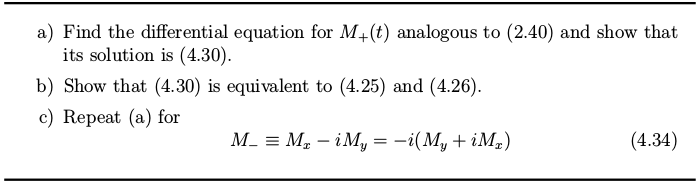
\includegraphics[width=0.8\textwidth,keepaspectratio]{prbl44}
    \label{fig:prbl44}
\end{figure}

\textit{Remember:}
\begin{itemize}
	\item The complex representation solutions.
\end{itemize}


\textit{a) Proof.}
%   \frac{d M_{+}}{dt} &= (-i \omega_0 - \frac{1}{T_2}) M_+ \\
%    \frac{d M_{+}}{dt} &= (-i \omega_0 - \frac{1}{T_2}) (M_x + i M_y) \\
%    \frac{d M_{+}}{dt} &= -i \omega_0 M_x + \omega_0 M_y - \frac{1}{T_2} M_x - \frac{i}{T_2} M_y \\
%    \frac{d M_{+}}{dt} &= i M_y(-i \omega_0 - \frac{1}{T_2}) + M_x (-\frac{1}{T_2} - i \omega_0) \\
%    \frac{d M_{+}}{dt} &= (-i \omega_0 - \frac{1}{T_2}) (M_x + i M_y) \\
% 
\begin{flalign*}
    \frac{d M_{+}}{dt} &= (-i \omega_0 - \frac{1}{T_2}) M_+ \\
    \frac{1}{M_{+}} d M_{+} &= (-i \omega_0 - \frac{1}{T_2}) dt \\
    \int_{M_{+}(0)}^{M_{+}(t)} \frac{1}{M_{+}} d M_{+} &= \int_{0}^{t} (-i \omega_0 - \frac{1}{T_2}) dt \\
    ln \frac{M_{+}(t)}{M_{+}(0)} &= t(-i \omega_0 - \frac{1}{T_2}) \\
    \frac{M_{+}(t)}{M_{+}(0)} &= e^{-i \omega_0 t - \frac{t}{T_2}} \\
    M_{+}(t) &= M_{+}(0) e^{-i \omega_0 t - \frac{t}{T_2}} \\
\end{flalign*}


\clearpage
%%%%%%%%%%%%%%%%%%%%%%%%%%%%%%
\Large{Problem 4.5}
\begin{figure}[H]
    \centering
    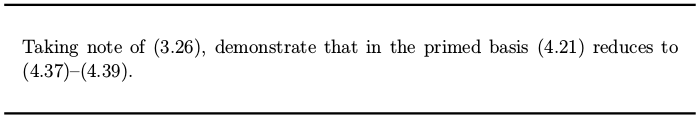
\includegraphics[width=0.8\textwidth,keepaspectratio]{prbl45}
    \label{fig:prbl45}
\end{figure}

\textit{Remember:}
\begin{itemize}
	\item The Bloch equations magnetization components in the primed basis.
\end{itemize}


\begin{figure}[H]
    \centering
    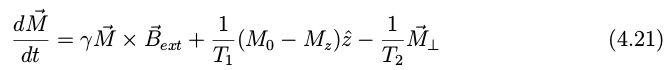
\includegraphics[width=0.8\textwidth,keepaspectratio]{form421}
    \label{fig:form421}
\end{figure}

\begin{figure}[H]
    \centering
    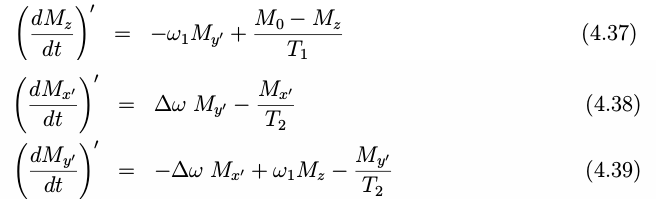
\includegraphics[width=0.8\textwidth,keepaspectratio]{form437438439}
    \label{fig:form437438439}
\end{figure}

\textit{Proof.}
\begin{flalign*}
    (\frac{d \vec{M}}{dt})' &= \gamma \vec{M}' \times \vec{B}_{eff} + \frac{1}{T_1} 
    (M_0 - M_z) \hat{z} - \frac{1}{T_2} (M_{x'} \hat{x}' + M_{y'} 
    \hat{y}') \\
    &= \gamma \vec{M}' \times [(B_0 - \omega / \gamma) \hat{z} + B_1 
    \hat{x}'] + \frac{1}{T_1} 
    (M_0 - M_z) \hat{z} - \frac{1}{T_2} (M_{x'} \hat{x}' + M_{y'} 
    \hat{y}') \\
    &= \gamma(B_0 - \omega / \gamma) (- M_{x'} \hat{y}' + M_{y'} 
    \hat{x}') + \gamma B_1 (- M_{y'} \hat{z} + M_{z} \hat{y}') \\
    &+ \frac{1}{T_1} 
    (M_0 - M_z) \hat{z} - \frac{1}{T_2} (M_{x'} \hat{x}' + M_{y'} 
    \hat{y}') \Rightarrow \\ 
    (\frac{d M_z}{dt})' &= -\omega_1 M_{y'} + \frac{M_0 - 
    M_z}{T_1} \\
    (\frac{d M_x}{dt})' &= (\omega_0 - \omega) M_{y'} - 
    \frac{M_{x'}}{T_2} \\
    (\frac{d M_y}{dt})' &= -(\omega_0 - \omega) M_{x'} + \omega_1 M_z - 
    \frac{M_{y'}}{T_2} \\
    & \Rightarrow \\
    (\frac{d M_z}{dt})' &= -\omega_1 M_{y'} + \frac{M_0 - 
    M_z}{T_1} \\
    (\frac{d M_x}{dt})' &= \Delta \omega M_{y'} - 
    \frac{M_{x'}}{T_2} \\
    (\frac{d M_y}{dt})' &= - \Delta \omega M_{x'} + \omega_1 M_z - 
    \frac{M_{y'}}{T_2} \\
\end{flalign*}

\clearpage
%%%%%%%%%%%%%%%%%%%%%%%%%%%%%%
\Large{Problem 4.6}
\begin{figure}[H]
    \centering
    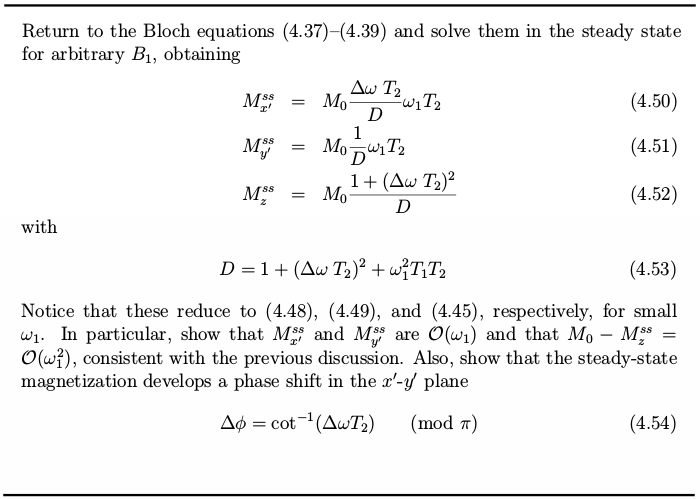
\includegraphics[width=0.8\textwidth,keepaspectratio]{prbl46}
    \label{fig:prbl46}
\end{figure}

\textit{Remember:}
\begin{itemize}
	\item    
\end{itemize}


\textit{Proof.}


